\documentclass[a4paperm]{article}
%\documentclass[12pt,twocolumn]{article}

\usepackage[T2A]{fontenc}
\usepackage[utf8]{inputenc}
\usepackage[russian,english]{babel}
\usepackage{amsmath,amsthm,amssymb,stackrel}
\usepackage[affil-it]{authblk}
\usepackage{cite}
\usepackage{scrextend}
\usepackage{verbatim}
\usepackage{paralist}
\usepackage[mediumspace,mediumqspace,Grey,squaren]{SIunits}
\addtokomafont{labelinglabel}{\sffamily}
\usepackage{amsmath}
\usepackage{graphicx}
 \usepackage[usenames, dvipsnames]{color}
 \usepackage{multirow}
 \usepackage{longtable}
 \usepackage{lineno}
 \usepackage{textcomp}
 
 \usepackage{xr}
 
 
%\usepackage[none]{hyphenat} %no nyphenation

\usepackage{SIunits}
\usepackage{miller}
\usepackage[version=3]{mhchem}

\usepackage{float} %H with figures

\setlength{\parindent}{5ex}

 \usepackage{newfloat} %For numbering of supplemmentary figures

\graphicspath{{figures/}}

\usepackage[outdir=figures/]{epstopdf}

\begin{document}

%\linenumbers


\title{Supporting Information}
\title{The Janus-structures of transition metal dichalcogenides with low enthalpy and new crystallchemistry}


\author[1,2,3]{Pavel N. Gavryushkin
   \thanks{Electronic address: \texttt{gavryushkin@igm.nsc.ru, p.gavryushkin@g.nsu.ru}; Corresponding author}}     
\author[2]{Nursultan Sagatov}
\author[1]{Ekaterina V. Sukhanova}
\author[1]{Zakhar I. Popov}
\author[4]{Inna Medrish}

\affil[1]{Emanuel Institute of Biochemical Physics of Russian Academy of Sciences, 4 Kosygin Street, Moscow, 119334, Russian Federation}
\affil[2]{Sobolev Institute of Geology and Mineralogy, Siberian Branch of Russian Academy of Sciences, prosp. acad. Koptyuga 3, 630090 Novosibirsk, Russian Federation}
\affil[3]{Novosibirsk State University, Pirogova 2, Novosibirsk 630090, Russian Federation}
\affil[4]{Samara Center for Theoretical Material Science (SCTMS), Samara State Technical University, Molodogvardeyskaya St. 244, Samara, Russia 443100}


\date{}
\maketitle

%\linenumbers

\begin{table}[H]
	\caption{Calculated enthalpies of MoS$_2$, MoSe$_2$, VS$_2$, and VSe$_2$ structures.} \label{t:enthalpy} \vspace{2mm}
	\centering
	\begin{tabular}{l*{10}{l}}
		\hline \hline
		\multirow{2}*{Phase} & \multicolumn{4}{c}{Enthalpy (eV/f.u.)} & & \multicolumn{4}{c}{Relative $\Delta$H (eV/f.u.)}	\\
		\cline{2-5} \cline{7-10}
		& MoS$_2$ & MoSe$_2$ & VS$_2$ & VSe$_2$ & & MoS$_2$ & MoSe$_2$ & VS$_2$ & VSe$_2$\\
		\hline    		
1H  	&	-21.7979	&	-19.9729	&	-16.6216	&	-14.9782	&	&	0.0000	&	0.0000	&	0.1225	&	0.2131	\\
1T  	&	-20.9517	&	-19.2645	&	-16.6942	&	-15.0745	&	&	0.8462	&	0.7085	&	0.0498	&	0.1168	\\
1T'	    &	-21.2477	&	-19.6420	&	-16.7440	&	-15.1913	&	&	0.5502	&	0.3309	&	0.0000	&	0.0000	\\
fes  	&	-20.9388	&	-19.2431	&	-16.1391	&	-14.5743	&	&	0.8591	&	0.7298	&	0.6049	&	0.6170	\\
fxt	    &	-20.8984	&	-19.2573	&	-16.0501	&	-14.5298   	&	&	0.8996	&	0.7156	&	0.6939	&	0.6615 	\\
test-1	&	-20.5707	&	-19.0322	&	-15.9051	&	-14.5779	&	&	1.2272	&	0.9408	&	0.8389	&	0.6134	\\
test-2	&	-21.0693	&	-19.4797	&	-16.1932	&	-14.7373	&	&	0.7287	&	0.4932	&	0.5509	&	0.4540	\\
test-3	&	-20.7775	&	-19.2060	&	-16.3075	&	-14.7683	&	&	1.0205	&	0.7669	&	0.4365	&	0.4230	\\
H-hor	&	-20.9226	&	-19.2149	&	-16.4369	&	-15.0158	&	&	0.8753	&	0.7581	&	0.3071	&	0.1755	\\
T-hor	&	-21.1194	&	-19.5238	&	-16.7402	&	-15.1292	&	&	0.6785	&	0.4491	&	0.0038	&	0.0621	\\
airss-1	&	-21.0882	&	-19.4064	&	-16.4716	&	-14.8615	&	&	0.7098	&	0.5665	&	0.2724	&	0.3298	\\
airss-3	&	-20.4745	&	-18.7452	&	-16.4849	&	-14.8839	&	&	1.3234	&	1.2278	&	0.2592	&	0.3074	\\

% Вот так выглядит последовательность структур в порядке увеличения энтальпии

% MoS2:  1H < 1T' < T-hor < airss-1 < test-2 < 1T < fes < H-hor < fxt < test-3 < test-1 < airss-3
% MoSe2: 1H < 1T' < T-hor < test-2 < airss-1 < 1T < fxt < fes < H-hor < test-3 < test-1 < airss-3
% SMoSe: 1H < 1T' < T-hor < test-2 < airss-1 < 1T < fes < H-hor < fxt < test-3 < test-1 < airss-3

% VS2:  1T' < T-hor < 1T < 1H < airss-3 < airss-1 < H-hor < test-3 < test-2 < fes < fxt < test-1
% VSe2: 1T' < T-hor < 1T < H-hor < 1H < airss-3 < airss-1 < test-3 < test-2 < test-1 < fes < fxt
% SVSe: 1T' < T-hor < 1T < 1H < H-hor < airss-1 < airss-3 < test-3 < test-2 < fes < fxt < test-1

		
		\hline \hline
	\end{tabular}
\end{table}


\begin{figure}[H]
	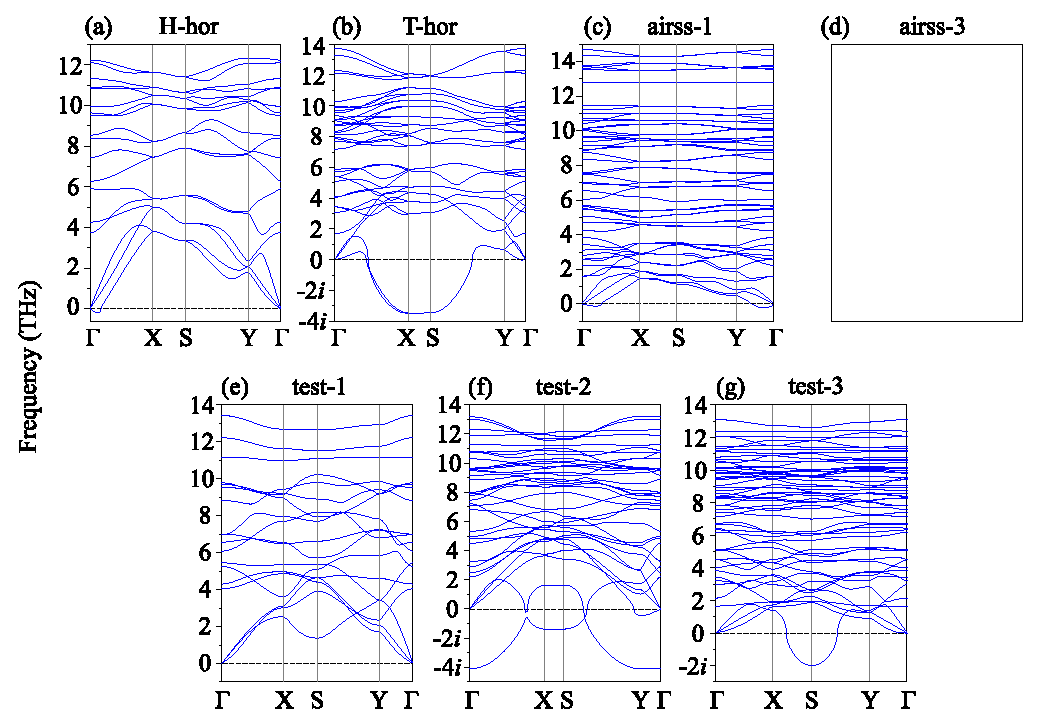
\includegraphics[width=\textwidth]{phon_mos2.eps}
	\caption{Phonon dispersion curves of MoS$_2$ structures. }
	\label{phon_mos2}
\end{figure}

\begin{figure}[H]
	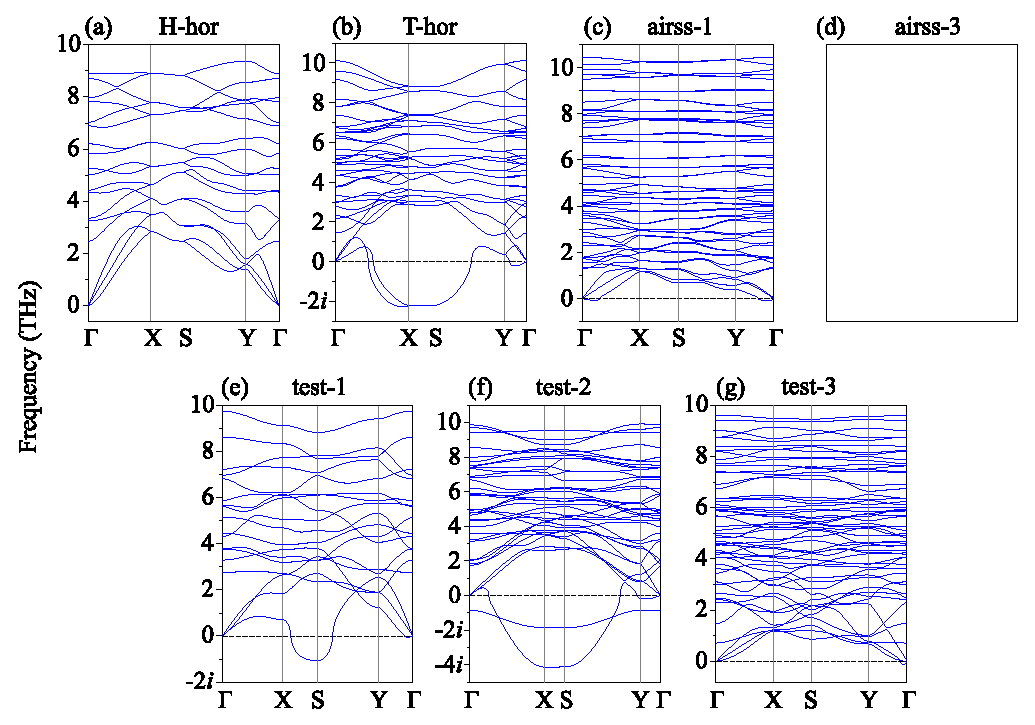
\includegraphics[width=\textwidth]{phon_mose2.eps}
	\caption{Phonon dispersion curves of MoSe$_2$ structures. }
	\label{phon_mose2}
\end{figure}

\begin{figure}[H]
	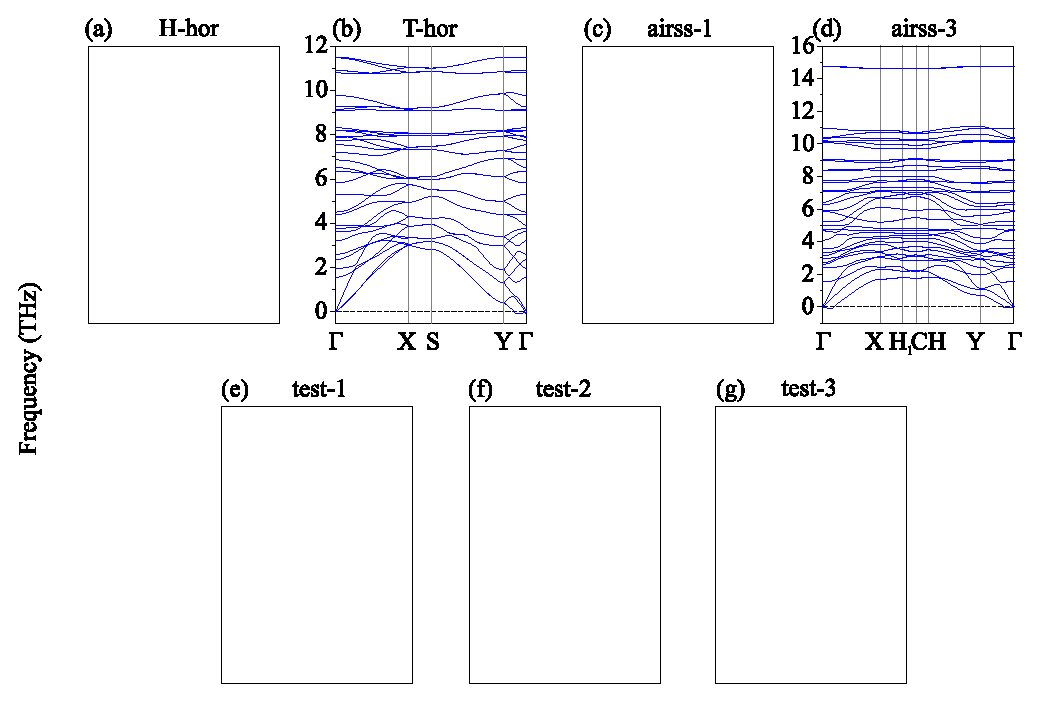
\includegraphics[width=\textwidth]{phon_vs2.eps}
	\caption{Phonon dispersion curves of VS$_2$ structures. }
	\label{phon_vs2}
\end{figure}

\begin{figure}[H]
	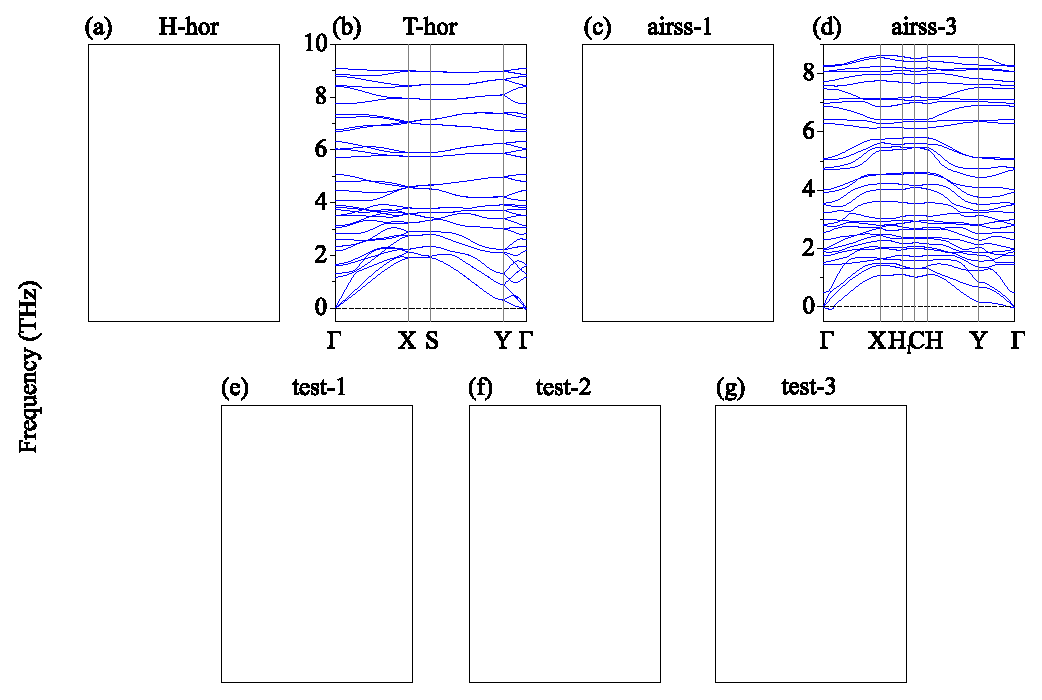
\includegraphics[width=\textwidth]{phon_vse2.eps}
	\caption{Phonon dispersion curves of VSe$_2$ structures. }
	\label{phon_vse2}
\end{figure}

\end{document}